\section{Discussion and Context Economics}
\label{sec:discussion}

\begin{figure*}[t]
\centering
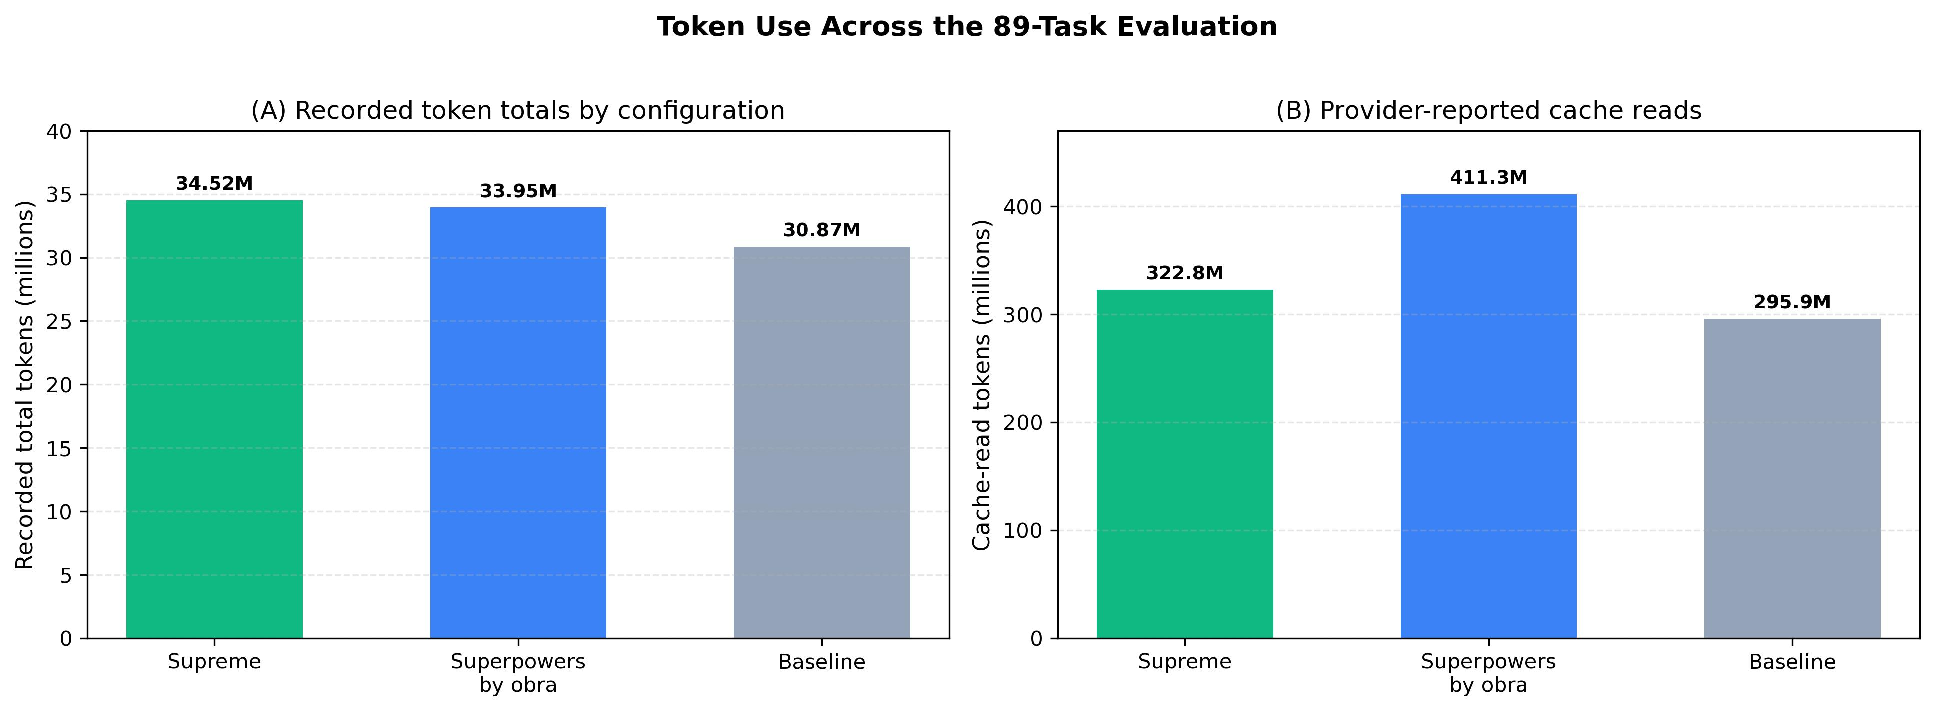
\includegraphics[width=\textwidth]{figures/fig4_token_usage_comparison.pdf}
\caption{Recorded token usage in the 89-task evaluation. (A) Recorded input-plus-output totals by configuration. (B) Provider-reported cache-read tokens, shown as a separate usage measure; the two panels are not additive components of one total.}
\label{fig:token_sinks}
\end{figure*}

\subsection{Context-Growth Dynamics and Multi-Turn Token Economics}
As illustrated in Figure~\ref{fig:token_sinks}, multi-turn agent execution exhibits distinctive context characteristics:
\begin{enumerate}
    \item \textbf{Input Share of Total Tokens}: For Supreme, input tokens comprised 90.5\% of recorded total tokens (31,232,870 / 34,521,410). This is an input-to-total ratio; it does not measure what share of input came from prior conversational history. In multi-turn runs, earlier conversation and tool outputs return as later-turn context, so initial prompt size alone does not describe full-trajectory input. Supreme's invariant header is approximately 7,000 tokens; Superpowers' initial discovery catalog is approximately 580 tokens and progressively loads procedural documents. These are different architectural layers: the comparison does not support describing Supreme as having the smaller initial context, nor does it quantify the complete skill-corpus sizes.
    \item \textbf{Observed Cache-Read Volume}: Provider-reported cache reads totaled \textbf{411,332,767 tokens} for Superpowers, 322,810,412 for Supreme, and 295,918,105 for Baseline \cite{google2026gemini36}. These are observed cache-read totals; this comparison does not isolate how much of the difference is attributable to dynamically loaded documentation.
    \item \textbf{Terminal Output in Tool Payloads}: Terminal stdout (including build logs and compiler output) represented 67.8\% of tool-payload tokens in the reported analysis. This points to output volume as a context-management consideration across configurations; it is not a measure of agent efficiency.
\end{enumerate}

\subsection{Financial Token Economics and Cost per Solved Task}
Table~\ref{tab:cost_economics} reports modeled API costs across the 267 evaluations under two rate schedules: the Gemini list-price reference (\$0.75 / M input, \$3.75 / M output) and the recorded OpenRouter rates (\$0.5598 / M input, \$3.745 / M output). These are rate-based estimates, not reported transaction charges.

\begin{table}[h]
\centering
\caption{Recorded token totals and rate-based cost estimates for the 267-evaluation study.}
\label{tab:cost_economics}
\resizebox{\columnwidth}{!}{%
\begin{tabular}{lccc}
\toprule
\textbf{Economic Dimension} & \textbf{Supreme} & \textbf{Superpowers} & \textbf{Baseline} \\
\midrule
Input Tokens ($T_{\text{in}}$) & 31.23M & 30.71M & \textbf{27.71M} \\
Output Tokens ($T_{\text{out}}$) & 3.29M & 3.25M & \textbf{3.16M} \\
Deliberation Tokens ($T_{\text{think}}$) & 1.83M & \textbf{1.71M} & 1.77M \\
Recorded Total Tokens (Input + Output) & 34.52M & 33.95M & \textbf{30.87M} \\
Cache Read Tokens ($T_{\text{cache}}$) & 322.8M & 411.3M & \textbf{295.9M} \\
\midrule
Modeled Total (List-Price Rates) & \$35.76 & \$35.21 & \textbf{\$32.62} \\
Modeled Cost / Successful Task (List) & \textbf{\$0.586} & \$0.607 & \$0.593 \\
\midrule
Modeled Total (OpenRouter Rates) & \$29.80 & \$29.35 & \textbf{\$27.33} \\
Modeled Cost / Attempted Task (OpenRouter) & \$0.335 & \$0.330 & \textbf{\$0.307} \\
Modeled Cost / Successful Task (OpenRouter) & \textbf{\$0.489} & \$0.506 & \$0.497 \\
Modeled Hard-Task Cost / Successful Task ($N=30$) & \$0.680 & \$0.730 & \textbf{\$0.645} \\
\bottomrule
\end{tabular}%
}
\end{table}
\par\smallskip{\footnotesize\noindent\emph{Note:} Component values are rounded independently; deliberation tokens are included in output and shown separately.\par}\smallskip

Across all 89 tasks, the rate-based cost estimates and outcomes present a three-layer economic portrait. Under the OpenRouter-rate model, Baseline had the lowest modeled total cost (\$27.33), followed by Superpowers (\$29.35) and Supreme (\$29.80). Baseline also had the lowest modeled cost per attempted task (\$0.307), followed by Superpowers (\$0.330) and Supreme (\$0.335). These modeled cost advantages coincide with Baseline's lower recorded token total (30.87M vs.\ 34.52M for Supreme), but also with its lower task completion (55/89 vs.\ 61/89).

Cost per successful task is a composite measure combining modeled total cost with the number of successful tasks; it is not a separately observed charge. On this measure, Supreme had the lowest modeled cost per successful task under the recorded OpenRouter rates (\$0.489), approximately 3.4\% below Superpowers (\$0.506), while completing three additional tasks (61 vs.\ 58). Baseline was \$0.497. The ranking is unchanged under both the list-price and OpenRouter-rate scenarios in Table~\ref{tab:cost_economics}.

On the Hard task subset ($N=30$), the cost-per-successful-task ranking reverses: Baseline achieved the lowest cost per successful Hard task (\$0.645), followed by Supreme (\$0.680) and Superpowers (\$0.730). Supreme simultaneously achieved the highest Hard-task completion rate (66.7\% [20/30] vs.\ 56.7\% [17/30] for Baseline and 53.3\% [16/30] for Superpowers), representing a genuine trade-off of superior Hard-task coverage at moderately higher cost per successful Hard solve compared to Baseline.

\subsection{Practical Design Implications for Agent Systems}
The evaluated configurations suggest three practical design considerations:
\par\textbf{Static Invariant Principles}: Static placement of invariant engineering principles can avoid mid-turn documentation retrieval while maintaining consistent behavioral constraints across turns.
\par\textbf{Loop Termination Heuristics}: Explicit iteration thresholds and hypothesis-checking gates help limit prolonged exploratory scripting on open-ended combinatorial problems.
\par\textbf{Targeted Line Edits}: Surgical diff tools (\texttt{replace\_file\_content}) correlate with reduced collateral modifications compared to whole-file rewrites.

\subsection{Threats to Validity and Limitations}
\textbf{Single Foundation Model}: All evaluations used Gemini 3.6 Flash High. Model-specific reasoning and tool policies may interact with prompt architecture; findings may not generalize across model families without multi-model replication.
\par\textbf{Single Run per Task}: Each task was evaluated with one run per configuration at $\tau=0.0$ (267 container runs, $\approx 50$ compute hours). While $\tau=0.0$ minimizes sampling variance, multi-seed replication is needed to measure run-to-run stability.
\par\textbf{Coupled Structure and Content}: Supreme and Superpowers differ in structure (static vs.\ dynamic) and content (constitutional axioms vs.\ TDD workflows). Controlled ablations isolating delivery mechanism from content remain future work.
\par\textbf{Prompt Freezing}: The Supreme constitutional prompt was frozen prior to benchmark execution; no prompt adjustments were made based on benchmark task failures.

\vspace{-0.3em}
\section{Conclusion}
\label{sec:conclusion}
Across the 89-task Terminal-Bench 2.1 evaluation (267 isolated container runs), the complete Supreme configuration recorded the highest task-completion rate (61/89, 68.5\%), the lowest aggregate wall-clock time (15.15\,h, 17.2\% below Superpowers), and the lowest modeled cost per successful task under recorded OpenRouter rates (\$0.489 vs.\ \$0.506 for Superpowers and \$0.497 for Baseline). Baseline had the lowest modeled absolute cost (\$27.33) and the lowest recorded token total (30.87M); Supreme's recorded total was 34.52M and Superpowers' was 33.95M. Supreme also recorded a directional lead on Hard tasks (20/30 vs.\ 16/30 for Superpowers and 17/30 for Baseline; paired McNemar $p = 0.22$). Aggregate completion differences were not statistically distinguishable under paired McNemar tests ($p > 0.05$). These results compare complete configurations with different guidance content and delivery mechanisms; they do not establish that static or dynamic delivery alone caused the observed differences. The evaluation provides an empirical baseline for this skill and benchmark; future work should replicate across model families and use controlled ablations to isolate design factors.

